\documentclass[
%a5paper,							% alle weiteren Papierformat einstellbar
%landscape,						% Querformat
12pt,								% Schriftgr��e (12pt, 11pt (Standard))
%BCOR1cm,							% Bindekorrektur, bspw. 1 cm
%DIVcalc,							% f�hrt die Satzspiegelberechnung neu aus s. scrguide 2.4
%twoside,							% Doppelseiten
%twocolumn,						% zweispaltiger Satz
%halfparskip*,				% Absatzformatierung s. scrguide 3.1
%headsepline,					% Trennline zum Seitenkopf	
%footsepline,					% Trennline zum Seitenfu�
%titlepage,						% Titelei auf eigener Seite
%normalheadings,			% �berschriften etwas kleiner (smallheadings)
%idxtotoc,						% Index im Inhaltsverzeichnis
%liststotoc,				  	% Abb.- und Tab.verzeichnis im Inhalt
listof=totoc,
%bibtotoc,			  			% Literaturverzeichnis im Inhalt
bibliography=totoc,
%abstracton,					% �berschrift �ber der Zusammenfassung an	
%leqno,   						% Nummerierung von Gleichungen links
%fleqn,								% Ausgabe von Gleichungen linksb�ndig
%draft								% �berlangen Zeilen in Ausgabe gekennzeichnet
]
{scrreprt}

\usepackage[T1]{fontenc}
\usepackage[ansinew]{inputenc}

\usepackage{amsmath}
\usepackage{amssymb}

%% ifthen f�r Vektordefinitionen
\usepackage{ifthen}

\usepackage{color}
\definecolor{blue}{rgb}{0,0,.8}
\definecolor{red}{rgb}{.8,0,0}
\definecolor{green}{rgb}{0,.8,0}
\definecolor{lightgray}{rgb}{0.9,0.9,0.9}

%% Formatierung f�r Listings
\usepackage{listings}
\lstset{
	keywordstyle=\color{blue}{\bfseries},
	stringstyle=\color{red},
	commentstyle=\color{green},
language=Java,                  % choose the language of the code
basicstyle=\footnotesize,       % the size of the fonts that are used for the code
numbers=left,                   % where to put the line-numbers
numberstyle=\footnotesize,      % the size of the fonts that are used for the line-numbers
stepnumber=2,                   % the step between two line-numbers. If it's 1 each line will be numbered
numbersep=10pt,                  % how far the line-numbers are from the code
backgroundcolor=\color{lightgray},  % choose the background color. You must add \usepackage{color}
showspaces=false,               % show spaces adding particular underscores
showstringspaces=false,         % underline spaces within strings
showtabs=false,                 % show tabs within strings adding particular underscores
frame=trbl,	                % adds a frame around the code
frameround=tttt,
tabsize=2,	                % sets default tabsize to 2 spaces
captionpos=t,                   % sets the caption-position to bottom
breaklines=true,                % sets automatic line breaking
breakatwhitespace=false,        % sets if automatic breaks should only happen at whitespace
%escapeinside={\%*}{*)}          % if you want to add a comment within your code
}

\usepackage{lmodern}

\usepackage{float}
\renewcommand{\bottomfraction}{1}
\renewcommand{\topfraction}{1}

%Kopf- und Fu�zeile---------------------------
\usepackage[automark, headsepline, plainheadsepline, footsepline, plainfootsepline]{scrpage2}
\pagestyle{scrheadings}
%\clearscrheadings
%\clearscrplain
%\lohead{\headmark}
%\rohead{}
%\lofoot{}
%\cofoot{\pagemark}
%\rofoot{}
%\setheadsepline{.4pt}
%\setfootsepline{.4pt}
%---------------------------------------------

%\usepackage{geometry}
%\typearea[current]{calc}
%\addtolength{\skip\footins}{8mm}
%\addtolength{\footnotesep}{2mm}
%\geometry{left=1.5cm,right=1.5cm,top=1cm,bottom=1cm}

\usepackage{graphicx} %%Zum Laden von Grafiken

\usepackage{natbib}

\parskip1.4ex
\parindent0pt

\def\pueb#1#2{\hspace*{-#1mm}{\buildrel{\hspace*{#1mm}
  \hspace*{#1mm} _\rightharpoonup}\over{#2}}\hspace*{-#1mm}
  \hspace*{-#1mm}\hspace*{-.2mm}}
\def\gpueb#1#2{\hspace*{-#1mm}\hspace*{.4mm}{\buildrel{
  \hspace*{#1mm}\hspace*{#1mm}{\displaystyle _\rightharpoonup}}
  \over{#2}}\hspace*{-#1mm}\hspace*{-#1mm}\hspace*{.4mm}}
\def\vc#1{
  \ifthenelse{\equal{#1}{f} \or \equal{#1}{d}}{\pueb{.4}{#1}}{
  \ifthenelse{\equal{#1}{e} \or \equal{#1}{k} \or \equal{#1}{l} 
    \or \equal{#1}{r} \or \equal{#1}{s} \or \equal{#1}{t} 
    \or \equal{#1}{\b} \or \equal{#1}{\beta} \or \equal{#1}{\ell} 
    \or \equal{#1}{\phi} \or \equal{#1}{\rho} 
    \or \equal{#1}{\varrho}}{\pueb{.2}{#1}}{   
  \ifthenelse{\equal{#1}{j}}{\pueb{.4}{\jmath}}{
  \ifthenelse{\equal{#1}{i}}{\pueb{.4}{\imath}}{
  \ifthenelse{\equal{#1}{m} \or \equal{#1}{w} \or \equal{#1}{\o}
       \or \equal{#1}{\omega}}{\gpueb{0}{#1}}{
  \ifthenelse{\equal{#1}{A} \or \equal{#1}{R}}{\gpueb{.2}{#1}}{
  \ifthenelse{\equal{#1}{B} \or \equal{#1}{C} \or \equal{#1}{D} 
 \or \equal{#1}{E} \or \equal{#1}{F} \or \equal{#1}{G} \or \equal{#1}{H} 
 \or \equal{#1}{I} \or \equal{#1}{J} \or \equal{#1}{K} \or \equal{#1}{L} 
 \or \equal{#1}{M} \or \equal{#1}{N} \or \equal{#1}{O} \or \equal{#1}{P} 
 \or \equal{#1}{Q} \or \equal{#1}{S} \or \equal{#1}{T} \or \equal{#1}{U} 
 \or \equal{#1}{V} \or \equal{#1}{W} \or \equal{#1}{X} \or \equal{#1}{Y} 
 \or \equal{#1}{Z}}{\gpueb{.4}{#1}}{\pueb{0}{#1}}} }}} }} }

%\usepackage{hyperref}

\begin{document}

\thispagestyle{empty}

\titlehead{{\Large Fachhochschule Hannover
\hfill WS 2010/11\\}
Fakult�t IV - Wirtschaft und Informatik\\
Ricklinger Stadtweg 118\\
30459 Hannover}
\subject{software requirements specification}
\title{\begin{center}
\includegraphics[width=0.55\textwidth]{images/genometa_logo.pdf}\end{center}}
%\subtitle{}
\author{FH Hannover}
%\date{\today}
\maketitle

\begin{table}
\begin{tabular}{|p{3.5cm}|p{3.5cm}|p{8cm}|}
\hline
\textbf{date}&\textbf{version}&\textbf{comments}\\
\hline
\today&0.1&initial release\\
\hline
\end{tabular}
\end{table}
\vfill

\tableofcontents

\chapter{Introduction}
This section gives a short introduction to the general scope of the project and ist primary goals.
\section{Purpose}
The SRS document is intended to represent a technical analysis of the product concept catalogue. It will try put the clients product specification into a technical perspective and to clarify main points for the programming staff.
\section{Scope}
In this project a software for visualizing DNA sequence reads is to be developed. The current project name "`genometa"' is subject for discussion and will be used as a preliminary name until a final name is decided upon.

The visualization will be useful in 2 distinct medical subcategories, namely in metagenomics - where bacteria are identified based upon their DNA - and transcriptomics - in which genes used by a specific bacterium are identified.

There are existing software products currently in use by the client, which only fulfill the requirements to a certain extent. The new software should incorporate the main advantages of these products and combine them into a single software solution.
\section{Definitions, Acronyms, and Abbreviations.}
The following definitions and abbreviations are used throughout this document
\begin{table}
\begin{tabular}{|p{3.5cm}|p{8cm}|}
\hline
\textbf{abbreviation}&\textbf{explanation}\\
\hline
DNA&short for deoxyribonucleic acid\\
$\vdots$&$vdots$\\
\hline
\end{tabular}
\end{table}
\section{References}
The following documents and other resources are referenced throughout this document
\begin{table}
\begin{tabular}{|p{2.5cm}|p{8cm}|p{4cm}|}
\hline
\textbf{reference}&\textbf{document}&\textbf{explanation}\\
\hline
PCC&lastenheft1.doc&product concept catalogue\\
\hline
SAMTools&http://samtools.sourceforge.net/SAM1.pdf&details about SAM format import/export\\
Picard&http://picard.sourceforge.net/index.shtml&alternative library for SAM/BAM import/export\\
IGB&http://www.bioviz.org/igb&Integrated Genome Browser\\
Geneious&http://www.geneious.com/&Geneious visualization program\\
Tablet&http://boiinf.scri.ac.uk/tablet/&Tablet visualization program\\
NGSView&http://ngsview.sourceforge.net/&NGSView visualization program\\
MagicViewer&&\\
SeqMonk&&\\
Apollo&&\\
\hline
\end{tabular}
\end{table}
\section{Overview}
The following chapters will give an a detailed description of the products functional and non-functional requirements and list the clients success criteria categorized to specific priority definitions.
\chapter{Project Description}
The genometa project will consist of a software implementation to visualize large datasets of DNA sequence reads in 2 different perspectives - metagenomics and transcriptomics. The current software packages used at MHH do not or only partially provide the tools needed for easy and efficient analyzation.
\section{Product Perspective}
Many software products have been listed as references by MHH and will be used to describe the specific advantages and disadvantages of each, hopefully defining an ideal software structure which will provide a complete package solution to the task that needs to be fulfilled.

The DNA sequence reads, which vary in sizes of around 10MB to 10GB will be provided in SAM format (Sequence Alignment/Map) and the corresponding binary format BAM. For importing and exporting these formats the SAMTools package as well as the Picard software library are provided.

The primary design goals will be an easy to use and visually appealing user interface as well as performance.
\subsection{Interfaces}
The system will be accesible to the user by means of a graphical user interface. A GUI design prototype will be presented in section.
\subsection{Hardware Interfaces}
The software is to be used on Windows, Linux and OS X platforms. Hardware is supposed to be on standard levels for office workspaces.
\subsection{Software Interfaces}
The source reads will be provided in SAM and BAM formatted files. The interfaces to read these files will be provided by either the SAMTools or Picard packages. A new import mechanism will be implemented if performance problems arise.
\subsection{Memory Constraints}
A total of 2GB to 4GB of RAM usage should not be exceeded.
\section{Product Functions}
This section will list the functional and non-functional requirements as specified in the product catalogue
\subsection{Functional requirements}
\subsection{Non-functional requirements}
\subsubsection{Priority 1}

\begin{tabular}{|p{7cm}|p{7cm}|}
\hline
\multicolumn{2}{|c|}{\textbf{Usability}}\\
\hline
\textbf{Functions in the program should be easily accessible to non-technically oriented biologist users.}
&
\begin{itemize}
	\item the software should provide a clear and understandable menu system
	\item an installation guide should be included
\end{itemize}
\\
\hline
\end{tabular}

\begin{tabular}{|p{7cm}|p{7cm}|}
\hline
\multicolumn{2}{|c|}{\textbf{Memory efficiency}}\\
\hline
\textbf{The program should be able to read between 0.1M and 100M reads from a SAM/BAM file into RAM rapidly. The memory usage should not exceed 4GB.}
&
\begin{itemize}
	\item the software should include a fast SAM/BAM importer/parser
	\item the software should provide a means of identifying the current memory usage (memory usage indicator)
\end{itemize}
\\
\hline
\end{tabular}

\begin{tabular}{|p{7cm}|p{7cm}|}
\hline
\multicolumn{2}{|c|}{\textbf{Multi processor capable}}\\
\hline
\textbf{The program should use multiple CPU cores if available.}
&
\begin{itemize}
	\item the following features should be parallelized if possible
	\begin{itemize}
	\item SAM/BAM import
	\item statistics generation
	\item graphics output (sliding window)
\end{itemize}
\end{itemize}
\\
\hline
\end{tabular}

\begin{tabular}{|p{7cm}|p{7cm}|}
\hline
\multicolumn{2}{|c|}{\textbf{Documentation}}\\
\hline
\textbf{The entire project should be documented.}
&
\begin{itemize}
	\item documentation should be provided for
	\begin{itemize}
	\item source code (doxygen)
	\item how to
	\item tips and tricks
\end{itemize}
\item all documentation will be in english
\end{itemize}
\\
\hline
\end{tabular}

\begin{tabular}{|p{7cm}|p{7cm}|}
\hline
\multicolumn{2}{|c|}{\textbf{Programming language}}\\
\hline
\textbf{The program code and any code for running external programs on the command line should be written in Java.}
&
\begin{itemize}
	\item the code will be written in SUN Java
	\item all external libraries and other dependencies will be thoroughly documented
\end{itemize}
\\
\hline
\end{tabular}

\subsubsection{Priority 2}

\begin{tabular}{|p{7cm}|p{7cm}|}
\hline
\multicolumn{2}{|c|}{\textbf{Platform independent}}\\
\hline
\textbf{The software should be usable on Windows, Linux and OS X systems.}
&
\begin{itemize}
	\item the software should be distributed my means of platform specific installer packages
	\item the software should be well organised and packaged
\end{itemize}
\\
\hline
\end{tabular}

\begin{tabular}{|p{7cm}|p{7cm}|}
\hline
\multicolumn{2}{|c|}{\textbf{Website}}\\
\hline
\textbf{A simple html/php website should be implemented for documentation and distribution of the program.}
&
\begin{itemize}
	\item the files and website will be hosted on MHH servers
	\item should include documentation and download pages
\end{itemize}
\\
\hline
\end{tabular}

\begin{tabular}{|p{7cm}|p{7cm}|}
\hline
\multicolumn{2}{|c|}{\textbf{Open source}}\\
\hline
\textbf{Software source code should be made available sometime in or after the main development process.}
&
\begin{itemize}
	\item the source code should be made available by means of an online codebase system (e.g. sourceforge) or as source file downloads
\end{itemize}
\\
\hline
\end{tabular}

\chapter{Time management}
The project will start in October 2010, and end on January 2011. On that date a stable product version should be made available included the defined documents and connected requirements (website, installer programs).

A preliminary time management plan is shown here:

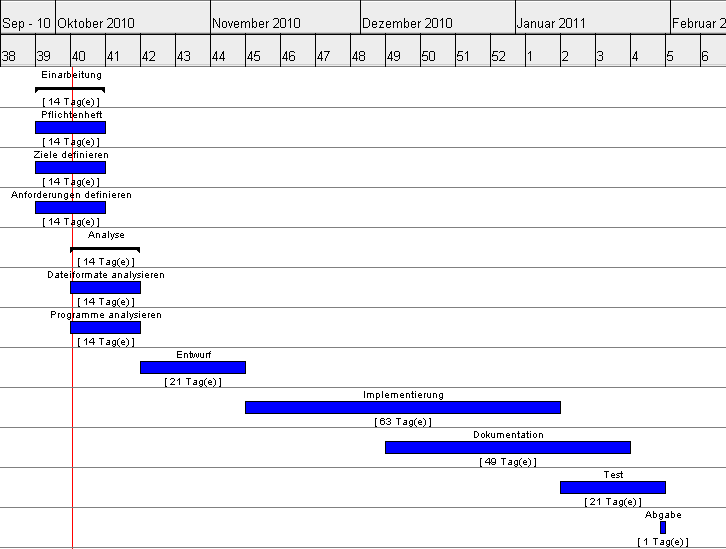
\includegraphics[width=\textwidth]{images/time_management.png}

The plan will be updated according to project revisions and definition of the work breakdown structure.

\end{document}